% 对偶空间：线性泛函、对偶空间与对偶基。

\section{线性泛函}
\label{sec:ls-dual-space}
\phantomsection
\label{sec:ls-dual-spaces}

\paragraph{线性泛函的定义}
保持线性组合的标量读取称为\term{线性泛函}（linear functional），即满足
\[
\varphi(a\bm x+b\bm y)=a\varphi(\bm x)+b\varphi(\bm y),\qquad\bm x,\bm y\in V,\ a,b\in\mathbb R
\]
的映射$\varphi:V\to\mathbb R$。它就是陪域为$\mathbb R$的线性映射。在$P_k$上，取值$p\mapsto p(t_0)$与积分$p\mapsto\int_0^1p(t)\,\mathrm dt$都是线性泛函；在$\mathbb R^d$上，读取第$j$个坐标与加权和$\bm x\mapsto\bm a^\top\bm x$都是线性泛函。但并非每个把向量读成一个数的规则都是线性泛函。
\begin{example}[反例：两个非线性的读取]
\label{ex:ls-nonlinear-readouts}
考虑$\mathbb R^d$上的两个读取：$\varphi_1(\bm x)=x_1+1$把第一个坐标加上$1$，$\varphi_2(\bm x)=\lVert\bm x\rVert_2$读出长度。线性泛函必把零向量读成$0$，而$\varphi_1(\bm0)=1$，常数项已经破坏了线性。$\varphi_2$在零向量处读数为$0$，问题出在符号上：线性泛函满足$\varphi(-\bm x)=-\varphi(\bm x)$，但对任一$\bm x\neq\bm0$，$\varphi_2(-\bm x)=\lVert\bm x\rVert_2>0$，而$-\varphi_2(\bm x)<0$。所以二者都不是线性泛函。
\end{example}

线性泛函是线性映射，所以也有矩阵表示。选定$V$的基$\mathcal B=(\bm b_1,\ldots,\bm b_d)$，输出端取数$1$作基，线性泛函$\varphi$记录为$1\times d$矩阵：
\[
 \begin{gathered}
[\varphi]_{\mathcal B}=\bigl(\varphi(\bm b_1),\ \ldots,\ \varphi(\bm b_d)\bigr)\\
\varphi(\bm v)=[\varphi]_{\mathcal B}[\bm v]_{\mathcal B}=\sum_{j=1}^dx_j\varphi(\bm b_j).
 \end{gathered}
\]
对象的坐标是一列，读取规则的系数是一行，二者相乘得到读数。

非零泛函的核与像也容易确定。非零泛函取到某个非零值，把相应的输入缩放即可取到任意实数，所以它的像是整个$\mathbb R$；由秩零度定理，它的核是$d-1$维子空间。读数等于$c$的点组成核的平移$\bm x_0+\ker\varphi$（其中$\varphi(\bm x_0)=c$），在平面上就是一族平行直线。

\paragraph{对偶空间}
同一个对象可以接受多种读取，两种读取也可以组合。规定
\[
 (\alpha\varphi+\beta\psi)(\bm x)=\alpha\varphi(\bm x)+\beta\psi(\bm x),
\]
右端对$\bm x$仍保持线性组合，所以线性泛函的线性组合仍是线性泛函。全部线性泛函在这两种运算下构成线性空间，称为$V$的\term{对偶空间}（dual space），记为$V^*$。输入向量是被读取的对象，泛函是读取规则，二者属于不同的空间。即使在$\mathbb R^d$中一行系数与一列坐标的数字相同，也不能把二者相加。

\paragraph{对偶基}
坐标给出了一组现成的读取，用它们可以确定$V^*$的维数。对$V$的有序基$\mathcal B=(\bm b_1,\ldots,\bm b_d)$，第$j$个坐标$\bm v\mapsto x_j$是线性泛函（坐标映射保持线性组合），记为$\varphi_j$。由于$\bm b_i$的坐标是$\bm e_i$，
\begin{equation}
 \varphi_j(\bm b_i)=\delta_{j,i}
 =\begin{cases}1,&i=j,\\0,&i\neq j.\end{cases}
 \label{eq:ls-dual-basis-def}
\end{equation}
反过来，线性泛函由它在基向量上的值决定，所以式~\eqref{eq:ls-dual-basis-def}也可以当作$\varphi_j$的定义。

这$d$个读取构成$V^*$的一组基。它们张成$V^*$：任意$\varphi\in V^*$都能写成
\[
 \varphi=\sum_{j=1}^d\varphi(\bm b_j)\,\varphi_j,
\]
因为两边在每个$\bm b_i$上取值都是$\varphi(\bm b_i)$，而线性泛函由基向量上的值决定。它们线性无关：若$\sum_ja_j\varphi_j=0$，在$\bm b_i$上取值得$a_i=0$。

$\varphi_1,\ldots,\varphi_d$称为$\mathcal B$的\term{对偶基}（dual basis），于是$\dim V^*=\dim V$。读取$\varphi$在对偶基下的坐标，正是它在各基向量上的读数$\varphi(\bm b_j)$，也就是上面那一行系数。

对偶基的每个成员依赖整组基，而不只依赖对应的那个基向量。
\begin{example}[改变第二个基向量会改变第一个坐标读取]
\label{ex:ls-dual-basis-depends-on-basis}
比较$\mathbb R^2$的标准基$(\bm e_1,\bm e_2)$与基$(\bm e_1,\bm e_1+\bm e_2)$，两者只有第二个向量不同。标准基的对偶基是两个坐标读取$\varphi_1(x,y)=x$、$\varphi_2(x,y)=y$。在第二组基下，把$(x,y)^\top$重新分解为
\[
 (x,y)^\top=(x-y)\bm e_1+y(\bm e_1+\bm e_2),
\]
所以第一个坐标读取变成$x-y$，第二个坐标读取仍是$y$。第一个基向量始终是$\bm e_1$，相应的对偶读取却从$x$变成了$x-y$。原因是新的第二个基向量也含有$\bm e_1$分量，第一个读取必须扣除由它贡献的那部分。
\end{example}
对一般的基，对偶基要由方程组$\varphi_j(\bm b_i)=\delta_{j,i}$解出。
\begin{example}[斜基的对偶基]
\label{ex:ls-dual-basis-oblique}
取$\mathbb R^2$的基$\bm b_1=(2,1)^\top$、$\bm b_2=(-1,1)^\top$，先求它的对偶基。线性泛函都形如$\varphi_1(x,y)=\alpha x+\beta y$，所以只需定出两个系数。条件$\varphi_1(\bm b_1)=2\alpha+\beta=1$与$\varphi_1(\bm b_2)=-\alpha+\beta=0$给出$\alpha=\beta=1/3$；同样由$\varphi_2(\bm b_1)=0$、$\varphi_2(\bm b_2)=1$解出$\varphi_2$，得
\[
 \begin{gathered}
\varphi_1(x,y)=\frac{x+y}3\\
\varphi_2(x,y)=\frac{-x+2y}3 .
 \end{gathered}
\]
再用这组对偶基表示读取横坐标的泛函$\ell(x,y)=x$。按前面的展开式，系数就是$\ell$在基向量上的读数$\ell(\bm b_1)=2$、$\ell(\bm b_2)=-1$，所以$\ell=2\varphi_1-\varphi_2$。代入验证：$\tfrac23(x+y)-\tfrac13(-x+2y)=x$。可见求读取在对偶基下的坐标不必解方程，只要把它作用在各基向量上。
\end{example}
图~\ref{fig:ls-dual-basis-readout}画出这些读取：每个对偶读取只在一个基向量上读到$1$，在另一个基向量上读到$0$。
\begin{figure}[htbp]
  \centering
  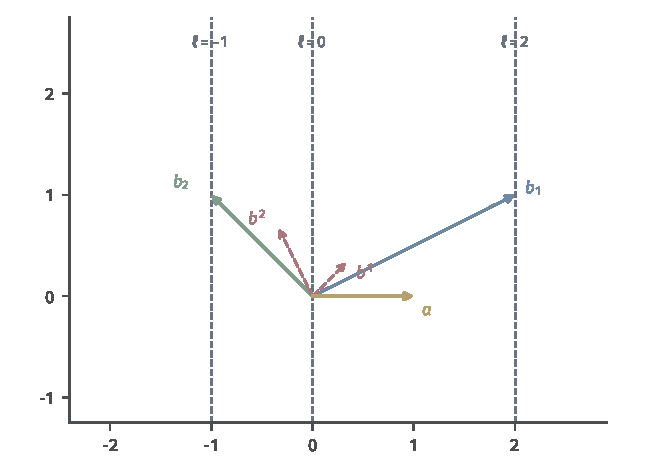
\includegraphics[width=112mm]{figures/00-shared/mathematical-preliminaries-upper/02-linear-spaces/matplotlib/ls-dual-basis-readout/ls-dual-basis-readout.pdf}
  \caption{对偶读取的几何示意。蓝箭头$\bm b_1=(2,1)$、绿箭头$\bm b_2=(-1,1)$为基向量；红色虚线箭头$\bm b^1=(1/3,1/3)$、$\bm b^2=(-1/3,2/3)$分别是对偶基$\varphi_1,\varphi_2$的系数向量，即$\varphi_i(\bm x)=\bm b^i\cdot\bm x$，满足$\varphi_i(\bm b_j)=\delta_{i,j}$。把读取规则画成平面箭头借用了标准内积，这一对应在第~\ref{sec:ls-riesz-representation}节说明。黄色箭头$\bm a=(1,0)$给出读取$\ell(\bm x)=\bm a\cdot\bm x$，灰色虚线为等值线$\ell=c$（$c=-1,0,2$）；$\ell(\bm b_1)=2$、$\ell(\bm b_2)=-1$，且$\bm a=2\bm b^1-\bm b^2$。}
  \label{fig:ls-dual-basis-readout}
\end{figure}

换基时，读取系数与坐标按相反的方向变化。设新基$\mathcal B'$由换基矩阵$\bm P=\bm S_{\mathcal B\leftarrow\mathcal B'}$给出，即$\bm b'_j=\sum_i\bm P_{i,j}\bm b_i$。坐标按
\[
 [\bm v]_{\mathcal B'}=\bm P^{-1}[\bm v]_{\mathcal B}
\]
变化；读取系数则按$\varphi(\bm b'_j)=\sum_i\varphi(\bm b_i)\bm P_{i,j}$变化，即
\[
 [\varphi]_{\mathcal B'}=[\varphi]_{\mathcal B}\bm P.
\]
二者相乘时$\bm P$与$\bm P^{-1}$相消，所以读数$\varphi(\bm v)$不随基改变，这正是读数应有的性质。
